\documentclass[12pt, a4paper]{article}
\usepackage[utf8]{inputenc}
\usepackage[russian]{babel}
\usepackage[T2A]{fontenc}
\usepackage{amsfonts}

\usepackage[left=2cm,right=1.5cm,top=2cm,bottom=2cm]{geometry}
\linespread{1.25}

\usepackage{graphicx}
\graphicspath{{pictures/}}
\DeclareGraphicsExtensions{.pdf,.png,.jpg}

\begin{document}
\section*{Тема}
Оптимизация транспортного потока при заданных пунктах отправления и назначения всех участников движения

\section*{Введение}

Данная дипломная работа посвящена одной из задач математического моделировнаия транспортных потоков. А именно нас интересует построение маршрутов при заданных координатах начала и конца движения на фиксированной карте дорожной сети. Целью является нахождение <<оптимальных>> путей, хотя выбор критерия оптимальности достаточно широк и неоднозначен, ведь участники влияют друг на друга и что хорошо для одного, может критически отразиться на движении другого. Мы предполагаем, что изначально дорожная сеть не содержит движущихся автомобильных транспортных (автотранспортных) средств (АТС) и наша задача, на самом деле, является задачей \textit{управления} транспортными потоками -- мы задаем направление движения каждого участника в каждый момент времени.



Говоря об актуальности задачи, достаточно сказать, что на данный момент существует множество научных журналов\footnote{Перечень научных журналов: Transportation Research B, Physical Review E, Review of modern physics, Transportation Science. Электронные ресурсы -- например, http://arxiv.org/}, в которых регулярно публикуются статьи на транспортную тематику. Также известное немецкое издательство Springer публикует труды ученых, представленных на конференции по математическому моделированию транспортных потоков «Traffic and granular flow», которая проводится с периодичностью в 2 года. Упомянутая конференция проходила и в Москве в 2011 году\footnote{На сайте https://link.springer.com/ можно ознакомиться с программой конференции.}. Также в столице регулярно проводится семинар\footnote{На следующих электронных ресурсах http://kozlov-traffic-ras.ru/, http://wtran.dvo.ru/ можно познакомиться с работами участников этого семинара.} «Научно-практические задачи развития автомобильно-дорожного комплекса в России» под руководством вицепрезидента РАН акад. В. В. Козлова.

Данная тема очень широка и включает в себя множество задач, таких как эволюция затора, задача о светофоре, задача о надежности графа транспортной сети и др. Наша задача затрагивает другие проблемы и входит в класс задач транспортного равновесия. Моделирование как задача принятия решений позволяет получить прогнозные оценки по загрузке элементов транспортной сети. Поставленная нами задача интересна тем, что она может служить инструментом для оценки эффективности проектов по модификации улично-дорожных сетей (УДС) с точки зрения разгрузки наиболее проблемных участков дорог и уменьшения общих затрат на передвижение пользователей сети.

Руководствуясь определенными принципами в теории транспортного равновесия, мы попробуем решить задачу построения оптимальных маршрутов итерационными методами, такими-то такими-то методами, не знаю, какими. 

Более подробно о постановке задачи вы сможете узнать в следующей главе, после чего следует описание возможных решений. В третьей главе мы посчитаем их сложность, зафиксируем положительные результаты исследования и проанализируем недостатки, подумаем над будущими улучшениями и другими решениями задачи. В конце оценим качество проделанной работы и подытожим результаты.

\newpage
\section*{Постановка задачи}

Пусть ориентированный граф $ G (V, E)$ задает дорожную сеть таким образом, что вершины $ v \in V$ осуществляют роль перекрестков, а ребра $e \in E$ - роль дорог. Длина ребер $l_e$ соответствует длине дороги, а кратность ребра $ k_e $ - количеству полос одностороннего движения, иначе говоря ширине дороги. 

Участники передвигаются со скоростями $v \in \mathbb {R}_{\geq 0}$, определенными зависимостью от расстояния до ближайшего спереди автомобиля и его скорости. Отметим, что все участники движения едут с максимально возможной скоростью, и она равна $ v_{max} \mathbb {R}_{\geq 0}$, если на движение автомомобиля ничего не влияет. Мы считаем, что автомобили могут останавливаться, т.е. нижней гранью скоркотси $ v $ выступает $v_{min} = 0$, причем теярть скорость участники могут сколько угодно быстро. Получаем $ 0 = v_{min} \leq v \leq v_{max} $.

Пусть в данной модели нам заданы $ n $ маршрутов - $ n $ последовательностей ребер. Требуется для $ n+1 $ водителя по заданным начальной и конечной вершинам определить оптимальный (наименьший по времени) путь и аремя его прохождения.

\newpage
\section*{Решения. Моделирование транспортных потоков}

стр 18-19


\newpage
\section*{Решения. Моделирование}

Узнать кратйчайший путь наверняка мы могли бы, если бы знали будущее. Это, конечно, невозможно в реальной жизни, но мы попробуем решить поставленную задачу путем моделирования дорожной ситуации. Мы знаем пути всех участников движения и можем рассчитать их скорости на каждом участке дороги в любой момент времени. Таким образом, получив информацию об усредненной скорости дорожного потока на ребрах мы сможем найти наилучший путь с хорошей(?) точностью.

Зададим некоторые условия на граф и движение автомобилей. 

\begin{enumerate}
	\item Очередь автомобилей на перекрестке формируется по времени приезда к вершине - кто первый приехал, тот первый в очереди.
	\item Пусть на ребрах задан приоритет - при встрече двух участников $ m_1 $ и $ m_2 $ на перекрестке, т.е. разница времени их подхода к перекрестку мала $ | t_{m_1} - t_{m_2} | < \varepsilon $, первым проезжает тот, на чьем ребре больший приоритет. Крытные ребра имеют одну и ту же степень приоритетности. 
	\item Если в начале движения количество автомобилей, движущихся в одном направлении, больше кратности ребра, то задаем время старта (какое кому и как?)
	\item После преодоления перекрестка, автомобиль выбирает то кратное ребро, на котором ближайший участник дальше всего.
\end{enumerate}

Будем считать, что скорость участника максимально, если ближайший перед ним участник находится на расстоянии $ s \geq D $, где $ D $-- заданная величина, например, 100 единиц.(?) Пусть отношение скорости от расстояния задано функцией $ f(s) $. необходимо понять с какой частотой пересчитывать сорости участников движения. Понятно, что при появлении или удалении участника на ребре, необходимо пересчитывать скоростиь однако помимо этого с течением времени автомобили меняют свою скорость при изменении расстоянии между друг другом.




\newpage
\section*{Алгоритм Дейкстры}

$\textbf{Неравенство прохождения ребер}$

Будем считать, что наша дорожная сеть обладает условием FIFO : чем позже въехать на дорогу, тем позже получится ее преодолеть (?).\\
Перенесем это на математический язык : \\
Пусть время прохождения по ребру задается формулой $f(t)$, где $t$ - время старта. Тогда получим, что $f(t) \le \Delta + f(t + \Delta)$, при $\Delta \ge 0$. Назовем это \textit{неравенством прохождения ребер}.


$\textbf{Алгоритм построения минимального маршрута}$

Для каждой вершины будем хранить два значения : минимальное время, за которое можно добраться до этой вершины, и ребро, через которое проходит кратчайший маршрут до вершины.
Если вес для ребра из вершины задается формулой $f(t)$,а минимальное время для этой вершины -- $x$, то за текущий вес ребра будем брать $f(x)$.
Применяем стандартный алгоритм Дейкстры, с отличием, что при посещении вершины мы фиксируем время для нее и пересчитываем текущий вес всех ребер (исходящих из этой вершины).\\
Для запуска алгоритма потребуется задать начальное время - минимальное время в точке старта. Это можно использовать в анализе маршрута.

$\textbf{Лемма}$

Данный маршрут обладает наименьшим временем прохождения.

$\textit{Док-во}$

Будем доказывать по индукции :\\
База индукции - в графе 2 вершины и несколько ребер между ними. Минимальным маршрутом будет то ребро, у которого наименьшее время прохождения.\\
Шаг индукции - считаем что в случае с m(< n) вершинами Лемма справедлива. Рассмотрим граф, содержащий n вершин. Пусть $\exists$ маршрут P в этом графе короче построенного нашим алгоритмом (будем пользоваться терминологией теории графов, хотя мы знаем, что ребра имеют вес-время вместо веса-длины), тогда возьмем ближайшую к началу точку, обозначим ее $C$, в которой выбрано ребро, не удовлетворяющее условию минимальности (?) из всех входящих. Очевидно, что если точка $C$ совпадает с точкой $F$, концом маршрута, то P не является минимальным по времени прохождения. \\
 Пусть ребро маршрута P в точку $C$ выходит из точки $B$, а минимальное - из точки $A$. Построим маршрут по нашему алгоритму из $S$ -- начала маршрута в $C$. Заметим, что он проходит через точку $A$. Обозначим время этого маршрута за $t_a = T(S-...-A-C)$, а время для части маршрута P из $S$ в $C$, проходящего через точку $B$, за $t_b = T(S-...-B-C)$. В подграфе $(P-C)$ вершин меньше чем n, а значит по индукции $t_a$ < $t_b$. 
\begin{center}
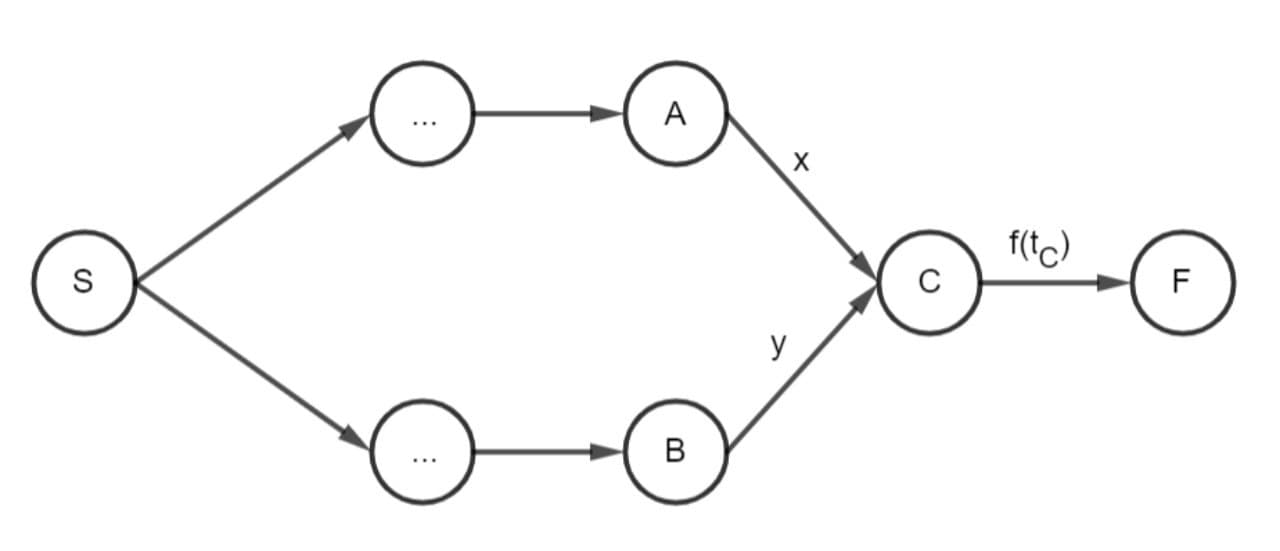
\includegraphics[scale=0.3]{graph_1.jpg}
\end{center}
\begin{center}
Рис 1.
\end{center}

Без ограничения общности, будем рассматривать часть маршрута P от точки C до F как одно ребро : C-F. Тогда обозначим время прохождения этого ребра как функцию $f(t_C)$, где $t_C$ - время старта из точки $C$. Вспомним неравенство прохождения для ребер (см. выше) : $f(t_a) \le (t_b - t_a) + f(t_b)$, где $\Delta = (t_b - t_a)$

Рассмотрим два маршрута $P : S-...-B-C-F$ и $P': S-...-A-C-F$.
Посчитаем время : $T(P) = t_b + f(t_b)$  и $T(P') = t_a + f(t_a)$
Используя неравенство, получаем : $T(P') = t_a + f(t_a) \le t_a + (t_b - t_a) + f(t_b) = T(P)$ Значит маршрут P не является минимальным. ЧТД


\newpage
\section*{Устойчивость нашего решения}



\newpage
\section*{Практические результаты}


\newpage
\section*{Сложность решения и альтернативные подходы}

\newpage
\section*{Заключение}

\newpage
\section*{Список литературы}

\end{document}